\documentclass{article}

\usepackage[%
    left=0.5in,%
    right=0.5in,%
    top=0.5in,%
    bottom=0.5in,%
]{geometry}%
\usepackage{minitoc}
\usepackage{multicol}
\usepackage{graphicx}
\usepackage{fixltx2e}
\usepackage{listings}
\usepackage{color}
\usepackage{hyperref}
    \hypersetup{ colorlinks = true, linkcolor = blue }
\usepackage{blindtext}
\definecolor{lightgray}{gray}{0.9}
\graphicspath{ {./} }

\newcommand{\inlinecode}[2]{\colorbox{lightgray}{\lstinline
[language=#1]$#2$}}
\newcommand{\worddef}[1]{\hyperref[sec:reference]{\textit{#1}}}

\begin{document}

\tableofcontents

\newpage

\section{Quality assurance and standards}
\begin{itemize}
  \item Standards may be international, national, organizational or project based
  \item Product standards define characteristics that all components should exhibit e.g. a common programming style and how the software process should be enacted
\end{itemize}

\subsection{Importance of standards}
\begin{itemize}
  \item Encapsulation of best practice – \textbf{avoids repetition} of past mistakes
  \item Framework for quality assurance process – it involves \textbf{checking standard compliance}
  \item \textbf{Provide continuity} – new staff can understand the organisation by understand the standards applied
\end{itemize}

\subsection{The benefits of using standards}
\begin{itemize}
  \item The ability to \textbf{apply methodologies and procedures} of the highest professional level.
  \item Better \textbf{mutual understanding} and coordination among development teams but especially between development and maintenance teams.
  \item \textbf{Greater cooperation} between the software developer and external participants in the project.
  \item Better understanding and cooperation between suppliers and customers, based on the adoption of standards as part of the contract
\end{itemize}

\section{SQM classes}

\begin{center}
  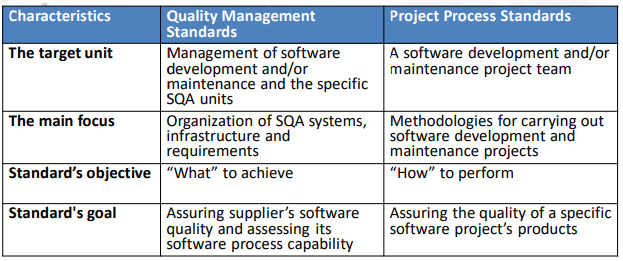
\includegraphics[scale=0.8]{sqa_classes.png}
\end{center}

\subsection{Certification standards}
\begin{itemize}
  \item Enable a software development organization to demonstrate \textbf{consistent ability} to assure acceptable quality of its software products or maintenance services. Certification is granted by an \textbf{external body}
  \item Serve as an agreed-upon basis for customer and \textbf{supplier evaluation} of the supplier’s quality management system. Accomplished by performance of a quality audit by the customer.
  \item Support the organization's efforts to improve its quality management system through compliance with the standard’s requirements.
\end{itemize}

\subsection{Assessment standards}

\begin{itemize}
  \item Serve organizations as a \textbf{tool for self-assessment} of their ability to carry out software development projects.
  \item Serve for \textbf{improvement of development} and maintenance processes by application of the standard directions
  \item Help purchasing organizations \textbf{to determine the capabilities} of potential suppliers.
  \item Guide training of assessor by \textbf{delineating qualifications and training program curricula}. its quality management system through compliance with the standard’s requirements.
\end{itemize}

\section{ISO 9000}
\begin{flushleft}
International set of standards for quality management. Applicable to a range of organisations from manufacturing to service industries. \textbf{ISO 9001}:
\end{flushleft}
\begin{itemize}
  \item is the current standard to which organisations can be certified
  \item applicable to organisations which design, develop and maintain products
  \item is a generic model of the quality process that must be instantiated for each organisation
\end{itemize}

\subsection{ISO 9001 Certification}

\begin{flushleft}
Quality standards and procedures should be documented in an organisational quality manual. \textbf{External body} may certify that an organisation’s quality manual conforms to \textbf{ISO 9001} standards. Customers are, increasingly, demanding that suppliers are \textbf{ISO 9001} certified
\end{flushleft}

\subsection{ISO 9001 principles}

\begin{itemize}
  \item Customer focus
  \begin{itemize}
    \item Understand the needs of existing and future customers
    \item Align organizational objectives with customer needs and expectations
    \item Meet customer requirements
    \item Measure customer satisfaction
    \item Manage customer relationships
    \item Aim to exceed customer expectations
  \end{itemize}
  \item Leadership
  \begin{itemize}
    \item Establish a vision and direction for the organization
    \item Set challenging goals
    \item Model organizational values
    \item Establish trust
    \item Equip and empower employees
    \item Recognize employee contributions
  \end{itemize}
  \item Involvement of people
  \begin{itemize}
    \item Ensure that people’s abilities are used and valued
    \item Make people accountable
    \item Enable participation in continual improvement
    \item Evaluate individual performance
    \item Enable learning and knowledge sharing
    \item Enable open discussion of problems and constraints
    \end{itemize}  
  \item Process approach
  \begin{itemize}
    \item Manage activities as processes
    \item Measure the capability of activities
    \item Identify linkages between activities
    \item Prioritize improvement opportunities
    \item Deploy resources effectively
  \end{itemize}
  \item Continual improvement
  \begin{itemize}
    \item Improve organizational performance and capabilities
    \item Align improvement activities
    \item Empower people to make improvements
    \item Measure improvement consistently
    \item Celebrate improvements
  \end{itemize}  
  \item Factual approach to decision making
  \begin{itemize}
    \item Ensure the accessibility of accurate and reliable data
    \item Use appropriate methods to analyze data
    e Make decisions based on analysis
    \item Balance data analysis with practical experienc
  \end{itemize}  
  \item Mutually supportive supplier relationships
  \begin{itemize}
    \item Identify and select suppliers to manage costs, optimize resources, and create value
    \item Establish relationships considering both the short and long term
    \item Share expertise, resources, information, and plans with partners
    \item Collaborate on improvement and development activities
    \item Recognize supplier successes
  \end{itemize}
\end{itemize}

\subsection{ISO 9001 – Requirements classification}
\begin{center}
  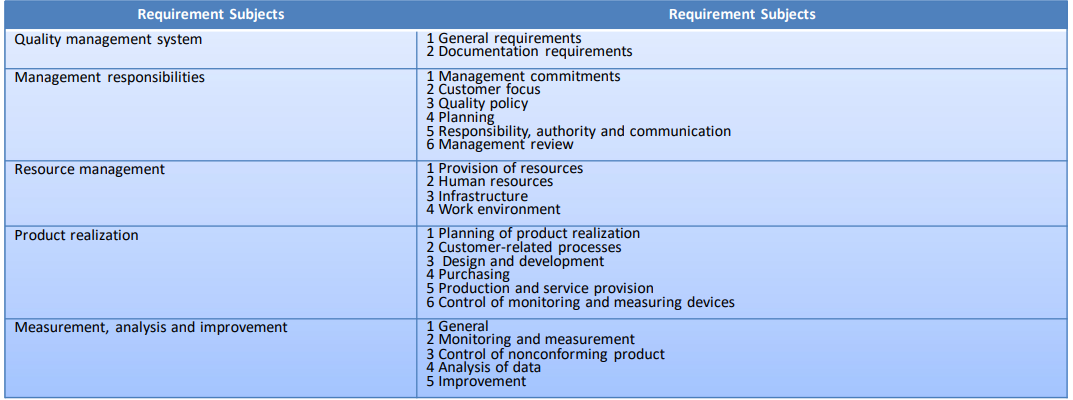
\includegraphics[scale=0.5]{requirements_classification.png}
\end{center}

\subsection{Certification Process}

\begin{center}
  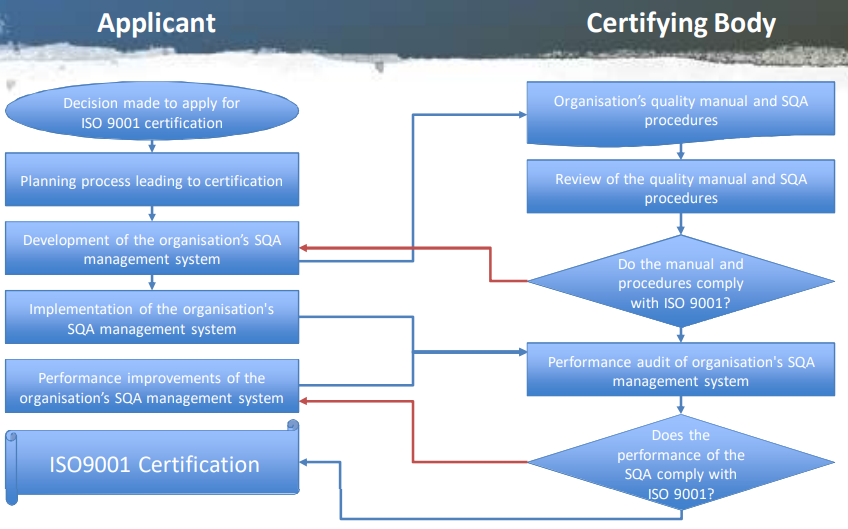
\includegraphics[scale=0.5]{certification_process.png}
\end{center}

\section{Capability Maturity Model (CMM)}
\begin{flushleft}
The Capability Maturity Model (CMM) is a methodology used to develop and refine an organization's software development process.
\end{flushleft}
\begin{itemize}
  \item Quantitative management methods increases the organization's capability to control the quality and improve the productivity.
  \item Application of the five-level capability maturity model that enables to evaluate the achievements and determine the efforts needed to reach the next capability.
  \item Generic process areas that define the “what” — not “how” enables the model's applicability to a wide range of implementation organizations:
  \begin{itemize}
    \item Allows use of any life cycle model.
    \item Allows use of any design methodology, development tool and programming language.
    \item Does not specify any particular documentation standard.
  \end{itemize}
\end{itemize}

\subsection{Structure}

\begin{center}
  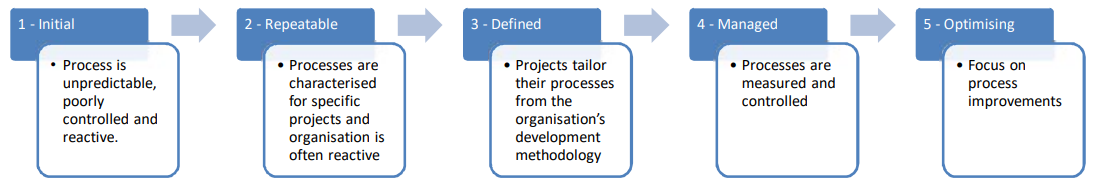
\includegraphics[scale=0.5]{cmm_structur.png}
\end{center}

\pagebreak
\section*{Reference section} \label{sec:reference}
\begin{description}
	\item[placeholder] \hfill \\
\end{description}
\end{document}
